\documentclass[tikz, margin=3mm]{standalone}
\usepackage{tikz}
\usepackage{amsmath}
\usepackage{comment}
\usetikzlibrary{shapes.geometric, arrows, positioning}
\tikzstyle{arrow} = [thick,->,>=stealth]

% flow chart of simulation (zoomed out view)
% uses relative positioning

% Terminal
\tikzstyle{terminal} = [rectangle, rounded corners, minimum width=3cm, minimum height=1cm,text centered, text width=3cm, draw=black]

% Process
\tikzstyle{process} = [rectangle, minimum width=3cm, minimum height=1cm, text centered,text width=4cm, draw=black]

% Decision
\tikzstyle{decision} = [diamond, aspect=1.8, minimum width=2cm, minimum height=1cm, text centered, text width=2cm, draw=black]

% Subprocess
\newcommand\ppbb{path picture bounding box}
\tikzset{
	subprocess/.style = {rectangle, draw=black, 
		minimum width=4.3cm, minimum height=1cm, inner xsep=3mm,
		text width =\pgfkeysvalueof{/pgf/minimum width}-2*\pgfkeysvalueof{/pgf/inner xsep},
		align=flush center,
		path picture={\draw 
			([xshift =2mm] \ppbb.north west) -- ([xshift= 2mm] \ppbb.south west)
			([xshift=-2mm] \ppbb.north east) -- ([xshift=-2mm] \ppbb.south east);
		},% end of path picture
	}
}

\tikzstyle{note} = [fill, ellipse,fill=gray!20, node distance=4cm, minimum height=1em, text width=3cm, text centered]

\begin{document}
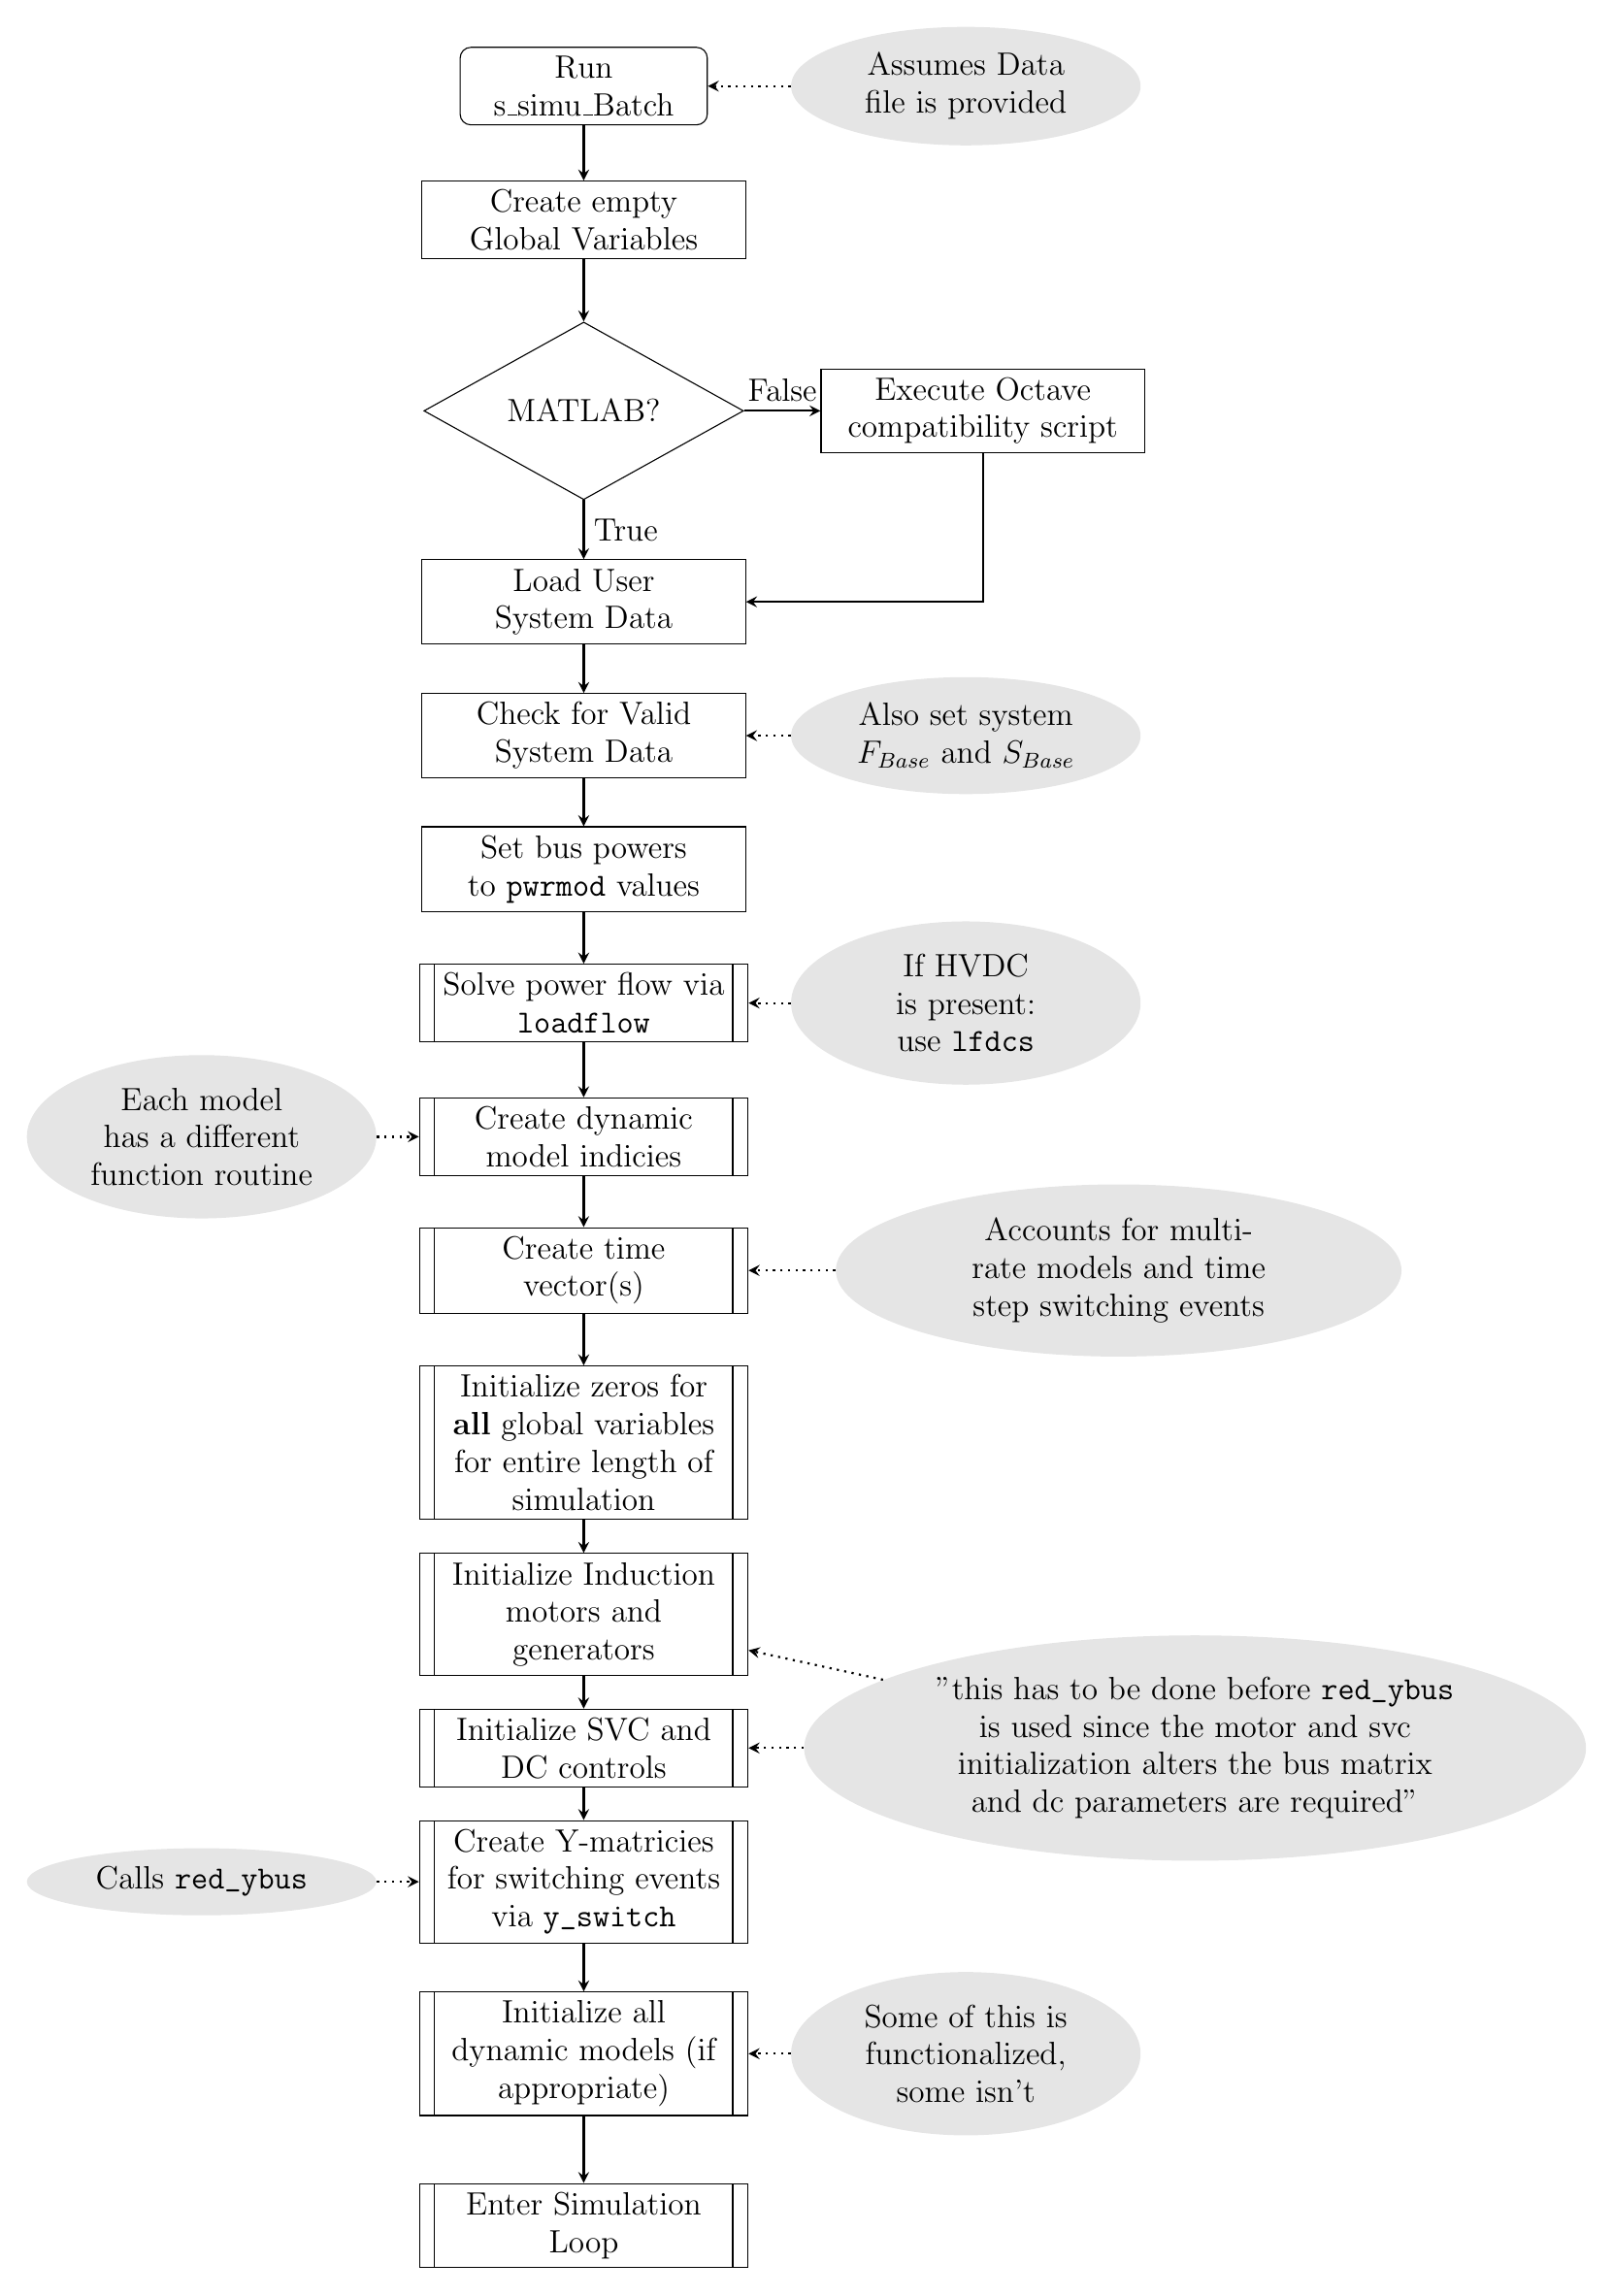
\begin{tikzpicture}[node distance=1.75cm, font=\large] 
% Placement of flowcart nodes
\node (start) [terminal] {Run s\_simu\_Batch};
\node (createGlobals) [process, below of = start] {Create empty Global Variables};
% matlab decision block
\node (checkProg) [decision, below of=createGlobals, yshift=-.75cm, text width=3cm] {MATLAB?};
\node (octaveComp) [process, right = 1 cm of checkProg] {Execute Octave compatibility script};

\node (loadData) [process, below of = checkProg, yshift=-.75cm] {Load User System Data};
\node (checkUserData) [process, below of = loadData] {Check for Valid System Data};
\node (pwrModInitCheck) [process, below of = checkUserData] {Set bus powers to \verb|pwrmod| values};
\node (initPF) [subprocess, below of = pwrModInitCheck] {Solve power flow via \verb|loadflow|};

\node (createModelIndicies) [subprocess, below of = initPF] {Create dynamic model indicies};
\node (createTimeVectors) [subprocess, below of = createModelIndicies] {Create time vector(s)};
\node (initializeZeros) [subprocess, below of = createTimeVectors, yshift=-.5cm] {Initialize zeros for \textbf{all} global variables for entire length of simulation};
\node (initInd) [subprocess, below of = initializeZeros, yshift=-.5cm] {Initialize Induction motors and generators};

\node (initSVCandDC) [subprocess, below of = initInd] {Initialize SVC and DC controls};
\node (createYswitch) [subprocess, below of = initSVCandDC] {Create Y-matricies for switching events via \verb|y_switch|};
\node (initDynamicModels) [subprocess, below of = createYswitch, yshift=-.5cm] {Initialize all dynamic models (if appropriate)};
\node (startSimLoop) [subprocess, below of = initDynamicModels, yshift=-.5cm] {Enter Simulation Loop};

% Drawing of Lines of main chart
\draw [arrow] (start) -- (createGlobals);
\draw [arrow] (createGlobals) -- (checkProg);
\draw [arrow] (octaveComp) |- (loadData);
\draw [arrow] (loadData) -- (checkUserData);

\draw [arrow] (checkUserData) -- (pwrModInitCheck);
\draw [arrow] (pwrModInitCheck) -- (initPF);
\draw [arrow] (initPF) -- (createModelIndicies);
\draw [arrow] (createModelIndicies) -- (createTimeVectors);
\draw [arrow] (createTimeVectors) -- (initializeZeros);

\draw [arrow] (initializeZeros) -- (initInd);
\draw [arrow] (initInd) -- (initSVCandDC);
\draw [arrow] (initSVCandDC) -- (createYswitch);
\draw [arrow] (createYswitch) -- (initDynamicModels);
\draw [arrow] (initDynamicModels) -- (startSimLoop);

% Draw Decision Lines
\draw [arrow] (checkProg) --  node[anchor=south] {False} (octaveComp);
\draw [arrow] (checkProg) --  node[anchor=west] {True} (loadData);

%% Note nodes AND edges
\node [note, right of=start, node distance =5cm](note1){Assumes Data file is provided};
\draw [arrow,dotted] (note1) -- (start);

\node [note, right of=checkUserData, node distance =5cm](note2){Also set system $F_{Base}$ and $S_{Base}$};
\draw [arrow,dotted] (note2) -- (checkUserData);

\node [note, right of=initPF, node distance =5cm](note3){If HVDC is present: use \verb|lfdcs|};
\draw [arrow,dotted] (note3) -- (initPF);

\node [note, left of=createModelIndicies, node distance =5cm](note4){Each model has a different function routine};
\draw [arrow,dotted] (note4) -- (createModelIndicies);

\node [note, right of=createTimeVectors, node distance =7cm,text width=5cm](note5){Accounts for multirate models and time step switching events};
\draw [arrow,dotted] (note5) -- (createTimeVectors);

\node [note, right of=initSVCandDC, node distance =8cm,text width=7cm](note6){"this has to be done before \verb|red_ybus| is used since the motor and svc
initialization alters the bus matrix and dc parameters are required"};
\draw [arrow,dotted] (note6) -- (initSVCandDC);
\draw [arrow,dotted] (note6) -- (initInd);

\node [note, left of=createYswitch, node distance =5cm](note7){Calls \verb|red_ybus|};
\draw [arrow,dotted] (note7) -- (createYswitch);

\node [note, right of=initDynamicModels, node distance =5cm](note8){Some of this is functionalized, some isn't};
\draw [arrow,dotted] (note8) -- (initDynamicModels);

\end{tikzpicture}

\begin{comment}
% Basic flowchart example
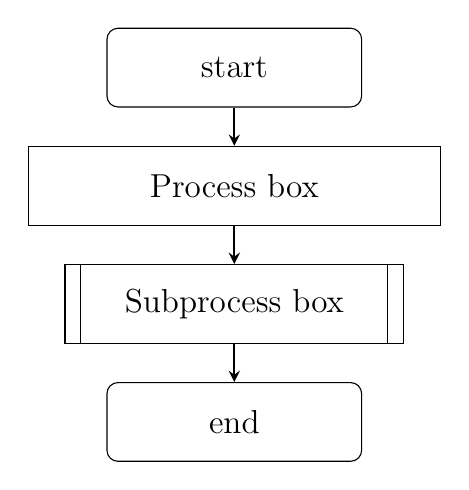
\begin{tikzpicture}[node distance=1.5cm, font=\large] 
% Placement of flowcart nodes
\node (term1) [terminal] {start};
\node (proc1) [process, below of = term1,text width=5cm] {Process box};% optional text width
\node (sproc1) [subprocess, below of = proc1] {Subprocess box};
\node (term2) [terminal, below of = sproc1] {end};

% Drawing of Lines
\draw [arrow] (term1) -- (proc1);
\draw [arrow] (proc1) -- (sproc1);
\draw [arrow] (sproc1) -- (term2);

\end{tikzpicture}


% Taken from PSLTDSim flowchart - here as a reference
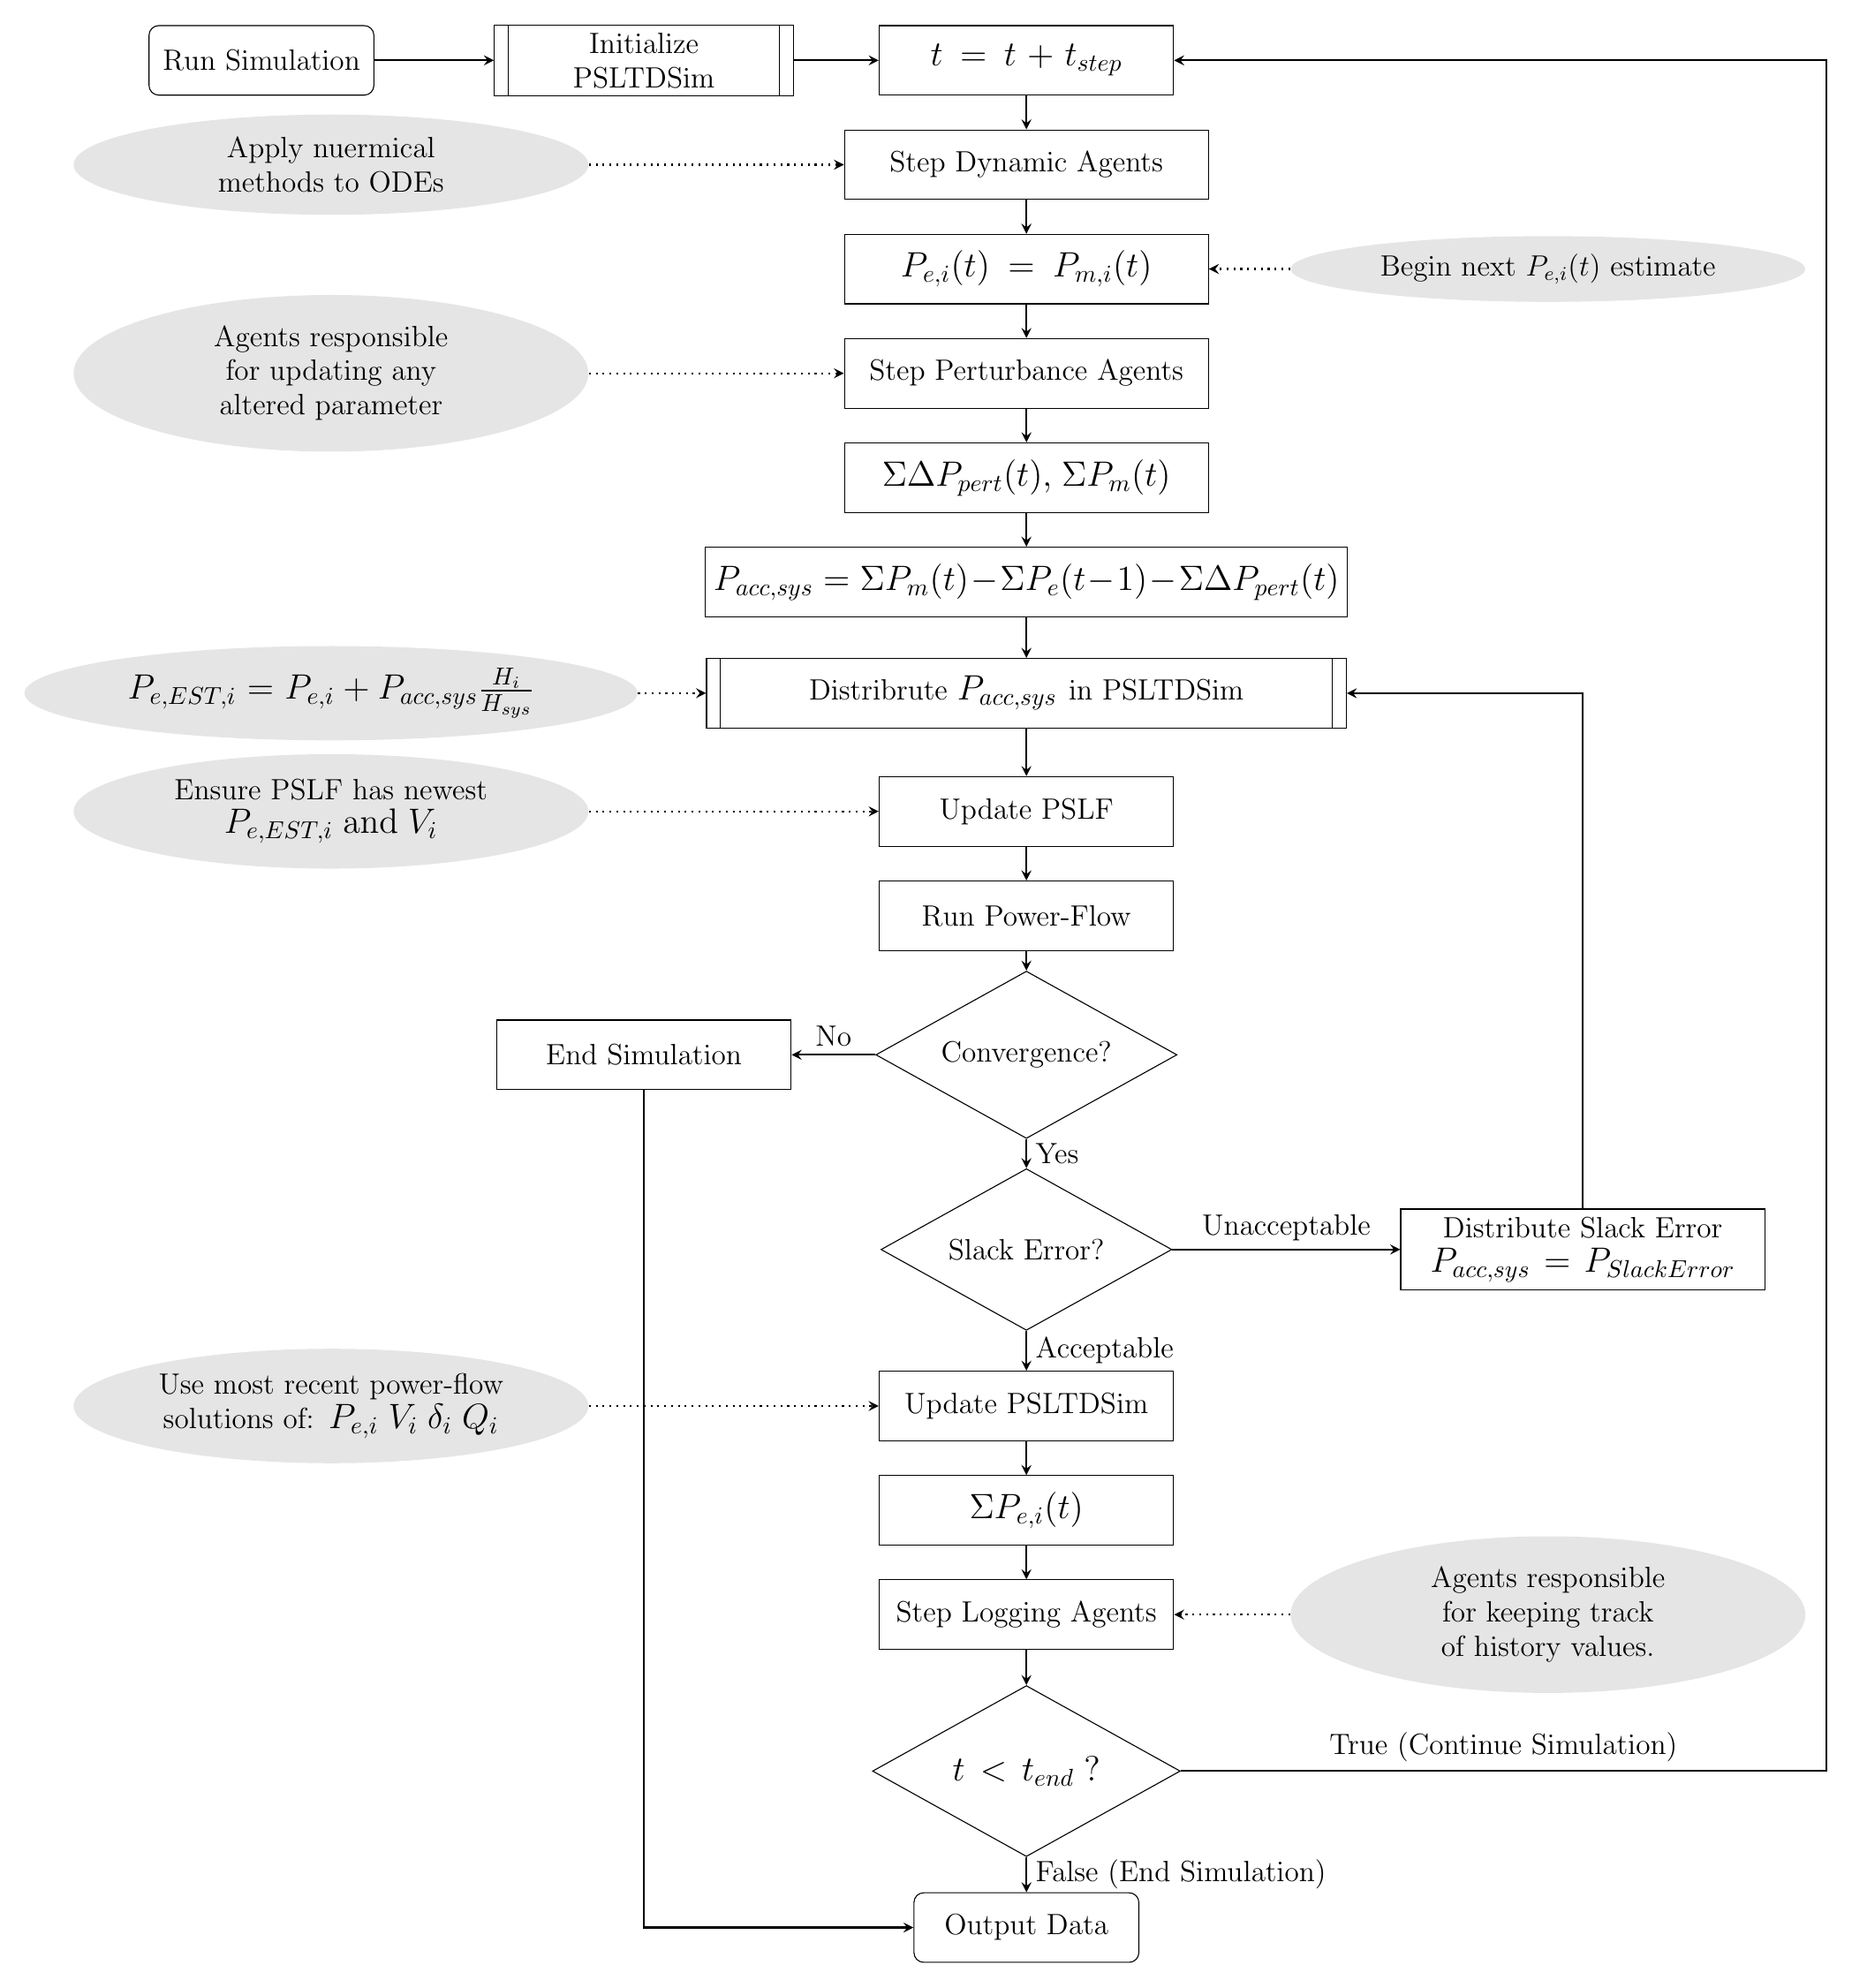
\begin{tikzpicture}[node distance=1.5cm, font=\large] 
% Placement of nodes
\node (start) [terminal] {Run Simulation};
\node (init) [subprocess, right of=start,xshift=4cm] {Initialize PSLTDSim};
\node (tStep) [process, right of=init,xshift=4cm] {\Large$t = t+t_{step}$};
\node (dyStep) [process, below of=tStep,text width=5cm] {Step Dynamic Agents};
\node (PeEst) [process, below of=dyStep,text width=5cm] {\Large$P_{e,i}(t) = P_{m,i}(t)$};
\node (stepPert) [process, below of=PeEst, text width=5cm] {Step Perturbance Agents};
\node (sumPertPm) [process, below of=stepPert, text width=5cm] {\Large$\Sigma\Delta P_{pert}(t)$, $\Sigma P_{m}(t)$};
\node (calcPacc)[process, below of=sumPertPm,  text width=9cm] {\Large$P_{acc, sys} = \Sigma P_m(t)-\Sigma P_e(t-1)- \Sigma \Delta P_{pert}(t)$};
\node (distPe) [subprocess, below of=calcPacc,yshift=-.1cm, text width=8.6cm] { Distribrute \Large$P_{acc, sys}$ \large in PSLTDSim};
\node (updatePSLF) [process, below of=distPe, yshift=-.2cm] {Update PSLF};
\node (runPF) [process, below of=updatePSLF,text width=4cm] {Run Power-Flow};

%Convergence nodes
\node (pfConv) [decision, below of=runPF, yshift=-.5cm, text width=3cm] {Convergence?};
\node (pfFail) [process, left of=pfConv, xshift=-4cm] {End Simulation};
%Slack error nodes
\node (slackErr) [decision, below of=pfConv, yshift=-1.3cm, text width=3cm] {Slack Error?};
\node (slackTol) [process, right of=slackErr, xshift=6.5cm, text width = 5cm] {Distribute Slack Error \\ \Large$P_{acc, sys} = P_{SlackError}$};

\node (updateLTD) [process, below of=slackErr,yshift=-0.75cm] {Update PSLTDSim};
\node (sumPe) [process,below of=updateLTD] {\Large$\Sigma P_{e,i}(t)$};
\node (log) [process, below of=sumPe, text width = 4cm] {Step Logging Agents};
\node (loop) [decision, below of=log, yshift=-.75cm, text width=3cm] {\Large$t<t_{end}$ ?};
\node (dataOut) [terminal, below of=loop, yshift=-.75cm] {Output Data};

%% Note nodes AND edges
\node [note, left of=updatePSLF, node distance =10cm,text width=5cm](note1){Ensure PSLF has newest \Large $P_{e,EST,i}$ and $V_{i}$};
\draw [arrow,dotted] (note1) -- (updatePSLF);

\node [note, left of=updateLTD, node distance =10cm, text width=5cm](note2){Use most recent power-flow solutions of: \Large $P_{e,i}\  V_i\  \delta_i \ Q_i$};
\draw [arrow,dotted] (note2) -- (updateLTD);

\node [note, left of=stepPert, node distance =10cm, text width=5cm](note3){Agents responsible for updating any altered parameter};
\draw [arrow,dotted] (note3) -- (stepPert);

\node [note, left of=dyStep, node distance =10cm, text width=5cm](note4){Apply nuermical methods to ODEs};
\draw [arrow,dotted] (note4) -- (dyStep);

\node [note, right of=PeEst, node distance =7.5cm, text width=5cm](note5){Begin next $P_{e,i}(t)$ estimate };
\draw [arrow,dotted] (note5) -- (PeEst);

\node [note, right of=log, node distance =7.5cm, text width=5cm](note6){Agents responsible for keeping track of history values.};
\draw [arrow,dotted] (note6) -- (log);

\node [note, left of=distPe, node distance =10cm, text width=6cm](note7){\Large$P_{e,EST,i}= P_{e,i} +P_{acc, sys}\frac{H_i}{H_{sys}}$};
\draw [arrow,dotted] (note7) -- (distPe);

% Placement of edges
\draw [arrow] (start) -- (init);
\draw [arrow] (init) -- (tStep);
\draw [arrow] (tStep) -- (dyStep);
\draw [arrow] (dyStep) -- (PeEst);
\draw [arrow] (PeEst) -- (stepPert);
\draw [arrow] (stepPert) -- (sumPertPm);
\draw [arrow] (sumPertPm) -- (calcPacc);
\draw [arrow] (calcPacc) -- (distPe);
\draw [arrow] (distPe) -- (updatePSLF);
\draw [arrow] (updatePSLF) -- (runPF);
\draw [arrow] (runPF) -- (pfConv);

% pf convergence bad
\draw [arrow] (pfConv) --  node[anchor=south] {No} (pfFail);
\draw [arrow] (pfFail) |-  (dataOut);
% pf convergence ok
\draw [arrow] (pfConv) --  node[anchor=west] {Yes} (slackErr);

% slack tolerance bad
\draw [arrow] (slackErr) --  node[anchor=south] {Unacceptable} (slackTol);
\draw [arrow] (slackTol) |- (distPe);
% slack tolerance ok
\draw [arrow] (slackErr) --  node[anchor=west] {Acceptable} (updateLTD);

\draw [arrow] (updateLTD) --(sumPe);
\draw [arrow] (sumPe) --(log);
\draw [arrow] (log) --(loop);

%loop again
\draw [arrow] (loop) -- node[anchor=south, midway] {True (Continue Simulation)} +(11.5,0) |- (tStep);
% end simulation
\draw [arrow] (loop) -- node[anchor=west] {False (End Simulation)} (dataOut);
\end{tikzpicture}
\end{comment}
\end{document}
